%xelatex
\documentclass[12pt]{article}

\usepackage[T2A]{fontenc}
\usepackage[english,ukrainian]{babel}
\usepackage{fontspec}
\setmainfont{Nimbus Roman}
\usepackage{graphicx}
\usepackage[a4paper,margin=0.5in]{geometry}
\pagestyle{empty}

\usepackage{pgfplots}% loads the package tikz
\pgfplotsset{compat=1.18}
\usetikzlibrary{intersections}
\usepackage{wrapfig}
\usepackage{pdfpages}
\usepackage{subfiles}

\begin{document}
\includepdf[pages=-]{5tit.pdf}
{\fontsize{14}{16.2}\selectfont

\subsection*{Мета роботи}
Експериментально перевірити основне рівняння динаміки обертального руху твердого тіла.

\subsection*{Прилади та обладнання}
Маятник Обербека, секундомір,  різноважки (тіла різної маси ), штанґенциркуль, міліметрова лінійка

\subsection*{Опис вимірювального пристрою, виведення
робочої формули}

Маятник Обербека (рис. \ref{mayatnik}) складається з чотирьох стрижнів (1), закріплених на втулці (2) під прямими кутами. Вздовж стрижнів можуть фіксовано пересуватися чотири однакові циліндри (3).

\begin{figure}[h]
	\centering
	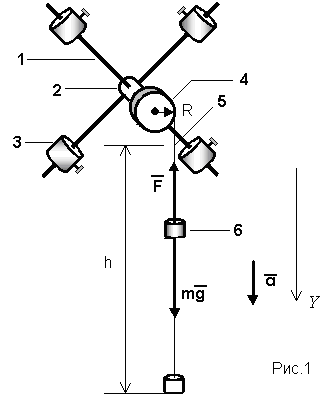
\includegraphics[width=5cm]{~/mayatniko.png}
	\caption{маятник Обербека\label{mayatnik}}
\end{figure}

Втулка і шків (4) радіуса  R  насаджені на спільний горизонтальний вал, що кріпиться у підшипниках до вертикального стояка. На шків намотується нитка (5), до кінця якої прикріплюються тіла (6) різних мас m (на основний вантаж можна накладати одну або дві різноважки).   Якщо обертальна система відцентрована, то поступальний рух тіл масою m і обертальний рух маятника будуть рівноприскореними.

\medskip

Другий закон Ньютона для тіла, яке опускається на нитці,
в проєкції н вісь Y (рис. \ref{mayatnik}):
$$m\alpha=mg-F,$$
де $F$ - сила натягу нитки.

Якщо експериментально виміряти час $t$  проходження тілом відстані $h$,
то з формули шляху рівноприскореного руху без початкової швидкості
можна обчислити  прискорення тіла:
$$\alpha = \frac{2h}{t^2}$$

Використавши зв’язок між танґенціальним прискоренням точок на ободі диску,
яке дорівнює прискоренню вантажу m, і кутовим прискоренням диску:
$$\alpha = \varepsilon \cdot R,$$
одержимо вираз для кутового прискорення маятника:
$$\varepsilon = \frac{2h}{t^2 R}$$

Обертальний момент сили, що викликає це прискорення:
$$M=FR=m\left(g-\frac{2h}{t^2}\right)R,$$
або через кутове прискорення:

$$M=m(g-\varepsilon R)R.$$

Отже, виконуючи експерименти з маятником Обербека, можна знаходити моменти сил, що діють на обертальну систему, та кутові прискорення системи.Оскільки крім моменту сили натягу нитки на систему діє ще момент сили тертя  M$_\textrm{т}$, то експеримент зведеться до перевірки рівняння:

$$M-M_\textrm{т} = J\varepsilon,$$

яке можна подати у вигляді:

$$\varepsilon=\frac{M-M_\textrm{т}}{J}.$$

З останньої формули видно, що залежності, які випливають з цього рівняння, $\varepsilon=f(M)$ та
$\varepsilon=\phi(1/J)$, повинні мати лінійний характер.

\subsection*{Задані величини}

$m_1 = 0.220$ кг,
$m_2 = 0.303$ кг,
$m_3= 0.386$ кг.

\subsection*{Фізичні величини, які вимірюються прямим способом}
$t$~--- час опускання вантажу, $d$~--- діаметр шківа, $h$~--- висота опускання тіла.

\subsection*{\centering{Таблиці результатів вимірювань та обчислень}}

\renewcommand{\arraystretch}{1.1}
\subsubsection*{\centering{Таблиця 1 (мін. момент інерції)}}

\begin{center}

	\subfile{1tab.tex}

\subsubsection*{\centering{Таблиця 1а}}
\begin{tabular}{|c| c| c| c| c| c| c| c|}
	\hline
	$h_1$, м & $h_2$, м & $h_3$, м & $h_{cep}$, м & $d_1$, м & $d_2$, м & $d_3$, м & $d_{cep}$, м\\
	\hline
	0.86 & 0.86 & 0.86 & 0.86 & 36.8 $\cdot$ 10$^{-3}$
	& 36.8 $\cdot$ 10$^{-3}$ & 36.8 $\cdot$ 10$^{-3}$
	& 36.8 $\cdot$ 10$^{-3}$\\
	\hline
\end{tabular}

\bigskip
Наступні величини обчислені за формулами $\varepsilon = \frac{2h}{t^2 R}$,
$M=FR=m\left(g-\frac{2h}{t^2}\right)R$, похибка для $\varepsilon$~--- за
формулою $\Delta\varepsilon=\left(\frac{\Delta h}{h}+\frac{\Delta R}{R}
+2\frac{\Delta t}{t}\right)\cdot\varepsilon$, $\Delta t =
\sqrt{\Delta t^2_{cep}+\Delta t^2_{np}}$

	\subfile{2tab.tex}

\subsubsection*{\centering{Таблиця 3}}

\begin{tabular}{|c|c|c|c|}
	\hline
	\No & $J$, кг м$^2$ & $\varepsilon$, с$^{-2}$ & $1/J$, кг$^{-1}$ м$^2$ \\
	\hline
	1 & 0.0166 & 2.6763 & 60.2409 \\
	\hline
	2 & 0.0338 & 1.2499 & 29.5857\\
	\hline
	3 & 0.0666 & 0.6024 & 15.015\\
	\hline
\end{tabular}

\end{center}

%\subsection*{Обчислення шуканої величини за робочою формулою}
$J_1=\frac{\Delta M_1}{\Delta \varepsilon_1}=\frac{2\cdot10^-2}{1.2}=0.01666$,
$J_2=\frac{\Delta M_2}{\Delta \varepsilon_2}=\frac{2\cdot10^-2}{0.59}=0.0338$,
$J_2=\frac{\Delta M_2}{\Delta \varepsilon_2}=\frac{2\cdot10^-2}{0.3}=0.06666$

%$M=mgR$

}


%{\fontsize{14}{16.2}\selectfont
\begin{center}
\subsection*{Графіки залежностей $\varepsilon$ від M (завдання 1)}

\subsubsection*{мін. момент інерції}

\subfile{plot.tex}

\subsubsection*{сер. момент інерції}

\subfile{plott.tex}

\subsubsection*{макс. момент інерції}

\subfile{plottt.tex}

\end{center}
%}

\newpage

\begin{center}

\subsection*{Графіки залежностей $\varepsilon$ від J та 1/J (завдання 2)}

\subsubsection*{графік залежності $\varepsilon$ від J}
\subfile{plot2mega.tex}

\subsubsection*{графік залежності $\varepsilon$ від 1/J}
\subfile{plot2ult.tex}

\end{center}

{\fontsize{14}{16.2}\selectfont
%\subsection*{Обчислення похибок}

\subsection*{Запис кінцевого результату}

\begin{itemize}
	\item $M_\textrm{т}=0.005$ --- для мінімального моменту інерції ($J=0.0166$);
	\item $M_\textrm{т}=0.004$ --- для середнього моменту інерції ($J=0.0338$);
	\item $M_\textrm{т}=0.0012$ --- для максимального моменту інерції ($J=0.0666$).
\end{itemize}

\subsection*{Аналіз кінцевих результатів та висновки}

	З виконанням цієї лабораторної роботи я отримав досвід
	роботи з маятником Обербека, навчився використовувати
	його для перевірки основного рівняння динаміки обертального
	руху твердого тіла. Аналізуючи побудовані графіки, дійсно,
	можемо пересвідчитись, що це рівняння має зміст.

	\newpage
	\hphantom{10pt}
\vspace{550pt}

Оцінка за виконання роботи:
\smallskip

\renewcommand{\arraystretch}{4}
\begin{tabular}{|c|c|c|}
	\hline
	\hspace{15pt} Допуск \hspace{15pt} & \hspace{15pt} Захист \hspace{15pt}
	& \hspace{15pt} Дата виконання \hspace{15pt}\\
	\hline
	 &  & \\
	\hline

\end{tabular}

\bigskip

	\begin{flushright}
		Підпис викладача:\line(1,0){70}\hspace{100pt}\hphantom{1pt}
	\end{flushright}
	}

\end{document}
